% !Mode:: "TeX:UTF-8"
% !TEX program  = xelatex
\documentclass[a4paper]{article}
\usepackage{amsmath}
\usepackage{amssymb}
\usepackage{ctex}
%\usepackage{braket}
%\usepackage[european]{circuitikz}
\usepackage{multirow}
\usepackage{float}
\usepackage{colortbl}
\usepackage{graphicx}
\usepackage{geometry}
\geometry{left=2.5cm,right=2.5cm,bottom=2.5cm,top=2.5cm}
\title{近代物理实验报告3.2:拉曼光谱}
\author{xy\quad 学号\quad 匡亚明学院}
\date{2019年2月29日}
\begin{document}
\maketitle
\bibliographystyle{unsrt}
%--------main-body------------

\section{引言}
拉曼光谱是分子或凝聚态物质的散射光谱。如果光线射向透明的液体、气体、固体,则将产生有部分的光不受物体表面的反射,而射入物体内部。当光和物体内的粒子发生碰撞时,就产生了散射现象。大部分的散射光子具有和入射光相同的频率,这种现象叫做弹性散射或瑞利散射。但有极少数的散射光具有不同的频率,这种现象叫做拉曼散射。以纪念第一位从实验上观察到这个现象的印度物理学家拉曼(C. V. Raman)。1928年拉曼以水银灯照射苯等液体后发现了这个效应,即在频率为$\omega$的瑞利散射线两侧对称地排列着数条拉曼散射偏振线,频率分别为$\omega_0-\omega$和$\omega_0-\omega$,其中$\omega$为介质的元激发频率,它们的频移量与红外振动频率相等。几乎与此同时,前苏联的物理学家曼杰斯塔姆(L. I. Mandelstam)和兰茨别尔格(G. S. Landsberg)在石英晶体中也观察到了类似的现象,它们是由光学声子引起的拉曼散射。拉曼因上述发现和他在分子散射方面的大量研究成果二获得1930年的诺贝尔物理学奖。

拉曼散射本质上是单色光与分子或晶体物质发生非弹性散射的结果。拉曼散射的发生是由于介质分子本身振动或转动,而造成入射光子和介质分子之间交换能量,使得散射光频率发生转变。振动拉曼谱线的数目、频移、强度直接与分子的振转能级有关。因此研究拉曼光谱可以有效的研究分子结构,分子振动能级、转动能级,分子中各种功能基或化学键位置的确定,以及复杂混合分子的定量分析和物质鉴定。除了已有的线性拉曼光谱技术,后来还发展了许多新的线性和非线性激光拉曼光谱技术。拉曼散射光谱技术是从事科研的重要工具,被广泛地应用于物理、化学、生物、地学、生命科学以及环境科学等研究领域。

\section{实验目的}
\begin{enumerate}
\item 掌握拉曼散射的基本原理,学会根据所测的拉曼散射光谱来辨别谱线的简正振动类型。
\item 掌握拉曼散射光谱的实验技术。
\end{enumerate}

\section{实验仪器}
激光拉曼光谱仪。

\section{实验原理}
当受光照射时,介质会对光产生散射。相对于入射光的频率或波数改变,可将散射分为三种类型。第一类是散射光的频率与入射光的频率差值小于3$\times 10^{5}$Hz,相应波数的差值小于$10^{-5}\text{cm}^{-1}$,通常称它为瑞利(Rayleigh)散射,第二类是频率变化约为3$\times 10^{9}$Hz,波数变化约为0.1cm$^{-1}$,称为布里渊(Brillouin)散射,第三类的频率会波数变化比较大,频率变化大于3$\times 10^{10}$Hz,波数变化比较大,频率变化大于3$\times 10^{10}$Hz,波数变化大于1cm$^{-1}$,这就是拉曼(Raman)散射。

从散射光的强度来看,瑞利散射最强,是入射光的$10^{-3}$左右,拉曼散射最弱,通常小于入射光的$10^{-6}$。因此当强度、单色性和方向性极好的激光的诞生,以及高质量、低杂散光的单色仪和高灵敏度的微弱信号检测系统出现以后,拉曼散射光谱技术才得以迅速发展。

实验得到的拉曼散射光谱图,其谱线有三个明显的特征:第一,拉曼散射光谱的波数$\widetilde{\nu}$随入射光的波数$\widetilde{\nu_0}$变化而变化,但对同一样品,同一拉曼线的波数差$\Delta\widetilde{\nu} = \widetilde{\nu} - \widetilde{\nu_0}$则保持不变;第二,在以波数为单位的拉曼光谱图上,$\Delta\widetilde{\nu}>0$的称反斯托克斯(Anti-Stokes)线;第三,一般情况下斯托克斯线的强度都大于反斯托克斯线。

下面,以$\text{CCl}_4$分子为例介绍拉曼散射的原理,并说明拉曼散射光谱与分子的结构、简正振动模式的对称性之间的关系。
\subsection{拉曼散射的经典解释}
在入射光场的作用下,介质分子将被诱发一个偶极矩。当入射光场不太强时,感应电偶极矩\textbf{P}与入射光电场呈线性关系
\begin{equation}
\textbf{P} = \alpha\cdot \textbf{E}\label{eq1}
\end{equation}
式中$\alpha$称为极化率,电场和偶极矩的方向如果均指向同一方向,极化率$\alpha$则为一纯量。通常情况\textbf{P}和\textbf{E}不在同一方向,因此\textbf{$\alpha$}是一个3$\times$3矩阵的二阶张量。
\begin{equation}
\textbf{$\alpha$} = 
\begin{bmatrix}
\alpha_{xx} & \alpha_{xy} & \alpha_{xz}\\
\alpha_{yx} & \alpha_{yy} & \alpha_{yz}\\
\alpha_{zx} & \alpha_{zy} & \alpha_{zz}
\end{bmatrix}\label{eq2}
\end{equation}
它通常是一个实对称矩阵,即有$\alpha_{ij} = \alpha_{ji}$,$\alpha_{ij}$的取值是由其具体介质的性质决定的,通常称部位零的$\alpha_{ij}$为拉曼活性的。

分子极化率张量\textbf{$\alpha$}是分子内部坐标的函数,如果分子中的原子在平衡位置附近振动,则振动分子的极化率将与平衡状态时的极化率不同。当振动幅度不大,即为简谐振动时,分子第k个振动的简正坐标可表示为
\begin{equation}
Q_k = Q_{k0}\cos(\omega_k+\Phi_k)\label{eq3}
\end{equation}
此时$\alpha_{ij}$将收到分子振动的微扰,它可用对简正坐标做泰勒级数展开表示
\begin{equation}
\alpha_{ij} = (\alpha_{ij})_0 + \sum\limits_{k}\left(\cfrac{\partial^2\alpha_{ij}}{\partial Q_k^2}\right)_0Q_k + \frac12\sum\limits_{k,l}\left(\cfrac{\partial^2\alpha_{ij}}{\partial Q_k\partial Q_l}\right)_0Q_kQ_l + \dots\label{eq4}
\end{equation}
式中右方第一项$(\alpha_{ij})_0$为零级项,它对应于分子处于平衡状态时的值,因而将对应不存在频移的瑞利散射。第二项中的$\left(\cfrac{\partial^2\alpha_{ij}}{\partial Q_k^2}\right)_0$是极化率对振动频率$\omega_0$的简正坐标的一级导数,表示在频率为$\omega_0$的简正振动中分子电极化率因微扰发生的变化,它将产生通常的(线性)拉曼散射。因此,拉曼散射,即拉曼活性,是同分子的而某个振动模式中电极化率是否发生变化相关联的,通常就称分子振动时导致电偶极矩发生变化的物质为“拉曼活性”的,与之相比,分子的红外光谱则是分子振动或转动中电偶极矩发生变化产生的,此时该物质称为“红外活性”的,拉曼散射光谱与红外光谱的实验技术和方法不同,不同分子或同一分子的振动和转动模式或者是拉曼活性,或者是红外活性的,因此两者相互结合互补,可以得到分子结构的而完整资料。

下面具体解释拉曼散射光谱。频率为$\omega_0$的入射光场可表示为
\begin{equation}
E = E_0\cos(\omega_0t)\label{eq5}
\end{equation}
它对分子产生的感应偶极矩为
\begin{eqnarray}
\textbf{P} 
&=& \alpha_{ij}\cdot\textbf{E} = (\alpha_{ij})_0E_0\cos(\omega_0t) + \left(\cfrac{\partial \alpha}{\partial Q_k}\right)_0Q_{k0}E_0\cos(\omega_0t)\cos(\omega_kt+\Phi_k)\nonumber\\
&=& \alpha_0E_0\cos(\omega_0t) + \frac12\left(\cfrac{\partial \alpha}{\partial Q}\right)_0Q_0E_0\cos[(\omega_0 - \omega_k)t+\Phi_k] + \frac12\left(\cfrac{\partial \alpha}{\partial Q}\right)_0Q_0E_0\cos[(\omega_0+\omega_k)t+\Phi_k]\nonumber\\
&=& P_0(\omega_0) + P_k(\omega_0 - \omega_k) + P_k(\omega_0 + \omega_k)
\end{eqnarray}
最后一等式中各项与前一等式中各项一一对应。它表明,入射光场对介质分子的极化作用将产生三个感应偶极矩,其频率$\omega_0$,$\omega_0 - \omega_k$,$\omega_0+\omega_k$,分别对应瑞利散射、斯托克斯拉曼和反斯托克斯拉曼散射。同时我们看到,具有简正振动的散射体的散射光场,可以视为入射光波被该散射提调制的结果。因此散射光波处仍以入射光频$\omega_0$辐射外,还产生与散射体振动频率$\omega_0$有关的差频$\omega_0 - \omega_k$及和频$\omega_0+\omega_k$的光。
\subsection{拉曼散射的量子解释}
在量子力学中,频率为$\omega_0$的入射单色光视作具有能量$\hbar\omega_0$的光子,与振动分子相互作用可视为碰撞过程。有两种碰撞:弹性碰撞和非弹性碰撞。在弹性碰撞中,不发生能量交换,光子只改变运动方向,这就是瑞利散射。非弹性碰撞则不仅改变光子的运动方向,而且发生能量交换,这就是拉曼散射。
\begin{figure}[!h]
\centering
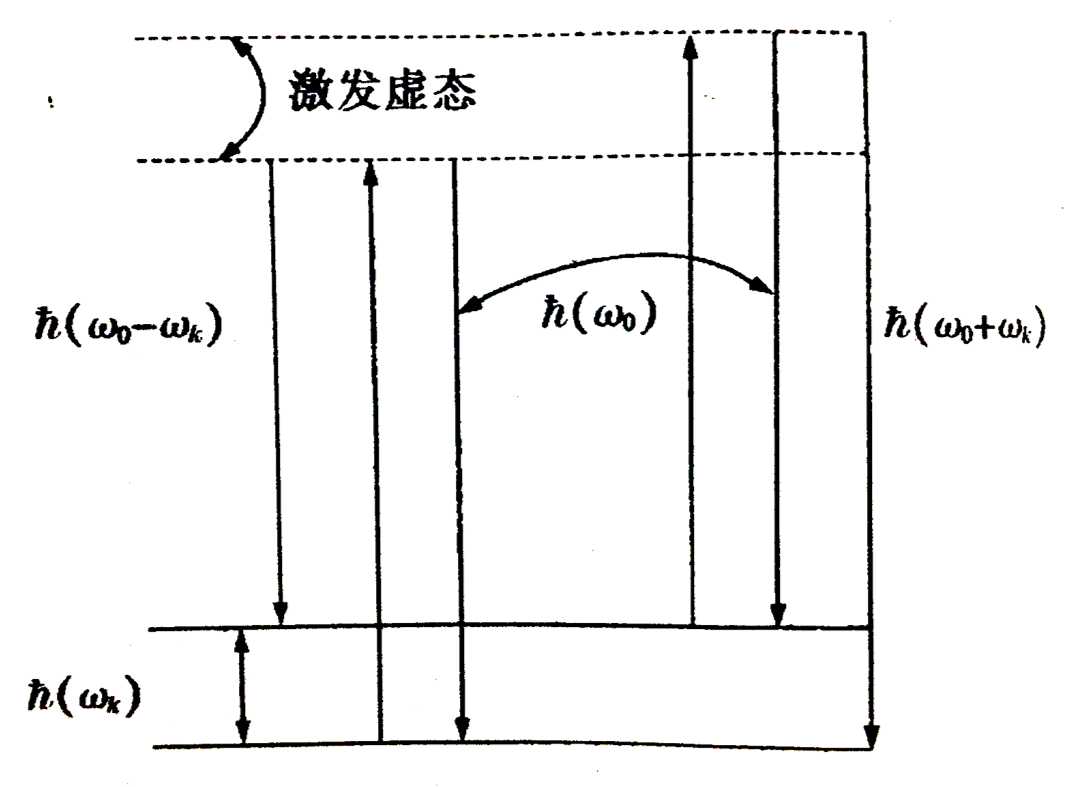
\includegraphics[width=10cm]{fig/1.png}\\
\caption{双原子分子拉曼散射能级跃迁图}\label{fig1}
\end{figure}
发生碰撞时,能量交换过程可用上面的能级跃迁图(图(\ref{fig1}))来说明。在基态和激发态均有大量分子,当它们受能量$\hbar\omega_0$的入射光子碰撞后,激发到各自的激发虚态。由于激发虚态不稳定,故立即自发向下越前,辐射一个光子。若光子能量仍为$\hbar\omega_0$,则分子仍回到初始能级,这即对应弹性碰撞的瑞利散射,若基态的分子通过碰撞后跃迁到激发态上,则辐射光的频率为$\hbar(\omega_0 - \omega_k)$,这种非弹性碰撞所产生的散射光为斯托克斯线;若激发态的分子通过碰撞跃迁到基态,则辐射光的频率为$\hbar(\omega_0+\omega_k)$,这种非弹性碰撞所产生的散射光为反斯托克斯线。

量子力学解释还可很好地说明斯托克斯线光强大于反斯托克斯线的问题。因为在热平衡时,各能级的分子束遵守玻尔兹曼分布律,该分子体系产生的斯托克斯线和反斯托克斯线的强度应分别对应各自能级上的分子数,因此两者的强度比是
\begin{equation}
\cfrac{I_{ks}}{I_{kas}} \approx e^{\frac{\hbar\omega_k}{k_BT}}\label{eq7}
\end{equation}
通常$e^{\frac{\hbar\omega_k}{k_BT}}\gg 1$,因而量子理论正确地这说明了斯托克斯线比反斯托克斯线强度大得多的问题。
\subsection{拉曼散射的偏振态和退偏度}
许多物质的分子通常有确定的空间取向,因此对某一分子而言,不论入射光是否是偏振光,该分子u的拉曼散射也将呈某种偏振状态,而且即使入射线偏振光,其散射光的偏振方向也通常不一定与其一致,他们之间的关系是由微商极化率张量$\left(\cfrac{\partial\alpha}{\partial Q_k}\right)_0$的具体形式确定的,因此对拉曼散射偏振状态的测量,可却日的那个分子结构的类型及其相应的振动方式。

然而在产生光散射的入射光照射区域中有大量的分子。每个分子虽然有确定的空间取向,但由于各个分子的空间取向不同,在宏观上则呈现无规分布,因此即使入射平面偏振光,整体散射光则是非完全偏振的,这一现象称为散射光的“退偏”,“退偏度”便是定量描述退偏程度的物理量。
\begin{figure}[!h]
\centering
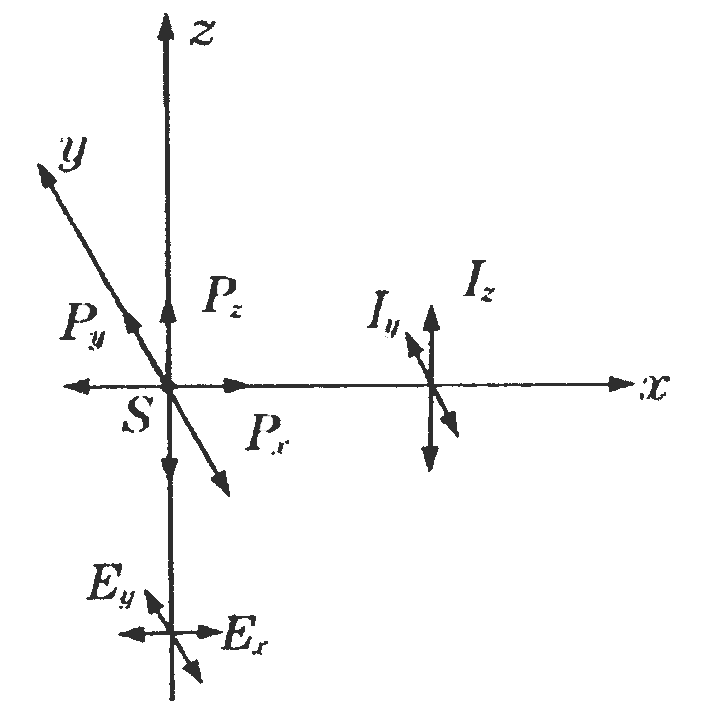
\includegraphics[width=8cm]{fig/2.png}\\
\caption{退偏比测量}\label{fig2}
\end{figure}
为了描述退偏度,可观察图(\ref{fig2})所示散射光的偏振示意图。入射光沿z轴传播,照射样品S上,使分子产生感应极化。当入射光为自然光时,有
$$E_z = 0,E_x = E_y \neq 0$$
分子产生的感应偶极矩为
$$P_x = \alpha_{xx}E_x+\alpha_{xy}E_y$$
$$P_y = \alpha_{yx}E_x+\alpha_{yy}E_y$$
$$P_z = \alpha_{zx}E_x+\alpha_{zy}E_y$$
若只探测沿x方向传播的散射光,则$P_x = 0$,只有$P_y$和$P_z$产生的散射光,它们的强度可分别用$I_y$和$I_z$表示,因为分子有某一可见取向,故同学$I_y$与$I_z$不相等。因此定义
\begin{equation}
\rho_n = \cfrac{I_y}{I_z}\label{eq8}
\end{equation}
为自然光入射时散射光的退偏振度,当入射光为线偏振光则用符号$\rho_p = \cfrac{I_y}{I_z}$表示。若入射光沿y方向传播,$E_x = 0$,$E_y \neq 0$,由于$E_y$与x方向散射光垂直,故用符号$\rho_{\perp}$表示,同理若入射光沿x方向偏振,即$E_x \neq 0$,$E_y = 0$,由于$E_x$平行于散射光的方向,故用符号$\rho_{\parallel}$表示。

理论计算已得各退偏度有如下结果:
\begin{eqnarray}
\rho_n &=& \cfrac{6\gamma^2}{45\bar{a}^2+7\gamma^2}\\\label{eq9}
\rho_{\perp} &=& \rho_{\parallel} = \cfrac{3\gamma^2}{45\bar{a}^2+4\gamma^2}\label{eq10}
\end{eqnarray}
式中$\bar{a}$称平均电极化率,$\gamma$称各向异性率,为极化率各向异性的量度。

实验测得的退偏度可判断分子振动的对称性。例如对某震动,当$\rho_{n} = \rho_{\perp} = \rho_{\parallel} = 0$时,即$I_y = 0$,表明此时散射是完全偏振的,因此分子的各向异性率$\gamma$必为零;当$\rho_n = \frac{6}{7}$,$\rho_{\perp} = \rho_{\parallel} = \frac{3}{4}$时,散射光是完全退偏的,表明平均极化率$\bar{a}$必为零;而当$0<\rho_n<\frac{6}{7}$,$0<\rho_{\perp} = \rho_{\parallel} = \frac{3}{4}$之间时,散射光就是部分偏振的。散射光的这种偏振特性反映了分子振动模式的对称性质。例如某个振动模式拉曼线的退偏度$\rho = 0$,则说明不管入射光是否为偏振光,它只激发感应偶极矩的$P_z$分量,而$P_z$得散射光在x-y评面2$\pi$角度内具有相同得最大强度,说明该振动必是对称振动。
\subsection{$\text{CCl}_4$(四氯化碳)分子的对称结构及振动模式}
本实验主要通过CCl$_4$分子的振动拉曼光谱,对其散射线的波数、数目及其偏振特性的研究,来分析该分子的对称结构及振动模式。
\subsubsection{CCl$_4$分子结构及其对称性}
该分子有一个碳原子和四个氯原子构成。它们构成正四面体结构(如图(\ref{fig3})),碳原子位于正四面体中心,四个氯原子位于正四面体的四个顶点。
\begin{figure}[!h]
\centering
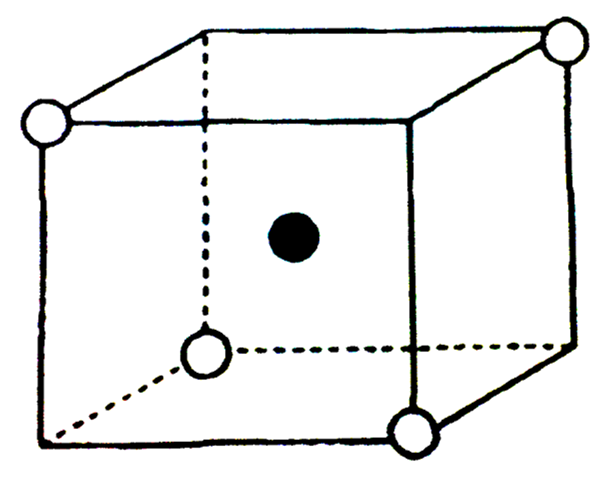
\includegraphics[width=4cm]{fig/3.png}\\
\caption{CCl$_4$分子结构图}\label{fig3}
\end{figure}
分子的对称性是指分子对应于某一几何元素(点、线、面)和进行某种操作后,所有源自在空间中的构型与操作前的构型是不可区分或者处于等价构型是,则称此分子具有该种对称性。CCl$_4$分子的构型属于Td群,即它有13跟对称轴,24个对称操作。这24个对称操作又可归属于5种对称素,对称素是分子对称性质的更简洁的表述。CCl$_4$分子的5中对称素是

E,3C$^m_2$,8C$^{j\pm}_3$,6iC$^p_2$,6iC$^{m\pm}_{4}$

这些对称素的含义是\\
E:不动操作。\\
$C_n$:旋转轴,下标n表示转角$\theta = \frac{2\pi}{n}$。\\
i:中心反演。\\
m:旋转轴方位是x,y,z轴。\\
j:旋转轴方位在远点的体对角线方向,j=1,2,3,4。\\
p:旋转轴方位在过远点O,立方体相对棱边中点连线方向,p=a,b,c,d,e,f。\\
$+$或$-$:顺时针或逆时针旋转方向。\\
每个对称素前的数字表示该对称素包含的对称操作数。
\subsubsection{CCl$_4$分子的振动模式及其拉曼谱}
由N个原子构成的分子由3N个自由度,出去3个平动自由度和3个转动自由度外,分子具有3N$-$6个振动自由度。因此CCl$_4$分子具有9个简正振动方式。根据分子的对称性,这9个简正振动可分为一下4类,在同一类中的各个震动方式具有相同的能量,即它们是简并的。
\begin{enumerate}
\item $\nu_1$或记为$A_1$:C原子不懂,Cl原子沿与C原子连线方向作伸缩振动,故此类振动只有一种振动方式。
\item $\nu_2$或记为$E$:C原子不动,一种是相邻两对Cl原子在与C原子连线方向上作相反振动,另一种是在该连线垂直方向上作相反振动,故此类振动是二重简并的。
\item $\nu_3$或记为$T_1$:四个Cl原子均作与C原子反向运动,由于是三维空间,故它是有三种振动方式的三重简并。
\item $\nu_4$或记为$T_2$:C原子不动,任意两对Cl原子组合,作伸张与压缩运动,由于是四个Cl原子,故它是由三种组合方式的三重简并振动。
\end{enumerate}
每一类简并对应同一条谱线,故CCl$_4$分子振动拉曼光谱由四条基频谱线(图(\ref{fig4}))。考虑到振动之间可能相互耦合引起的微扰,有的谱线可分裂为两体哦啊,这就是CCl$_4$拉曼谱中最弱线分裂成两体哦啊的原因。根据实验,测得它们的强度依次为$\nu_1>\nu_4>\nu_2>\nu_3$。

与CC1$_4$分子结构类似的AB$_4$类分子,由于它们具有相同的空间结构与对称性,故拉曼光谱的基本面貌与特征,包括拉曼光谱线数目,强度、退偏度等都具有类似性。因而可以运用这种类似性,将一个结构未知的分子的拉曼光谱与结构已知的分子拉曼光谱进行比对,以确定该分子的结构及其对称性。然而应该指出的是,虽然它们的分子结构可能相同,但在不同分子中其原子、原子间距以及原子间的相互作用必然存在某些差异,因而它们的拉曼光谱在细节上是有差异的。此外,外界条件的变化也会对分子结构和运动产生影响,进而使其拉曼光谱产生相应的变化,因此拉曼光谱也可用来研究物质的浓度、温度和压力等的效应。
\begin{figure}[!h]
\centering
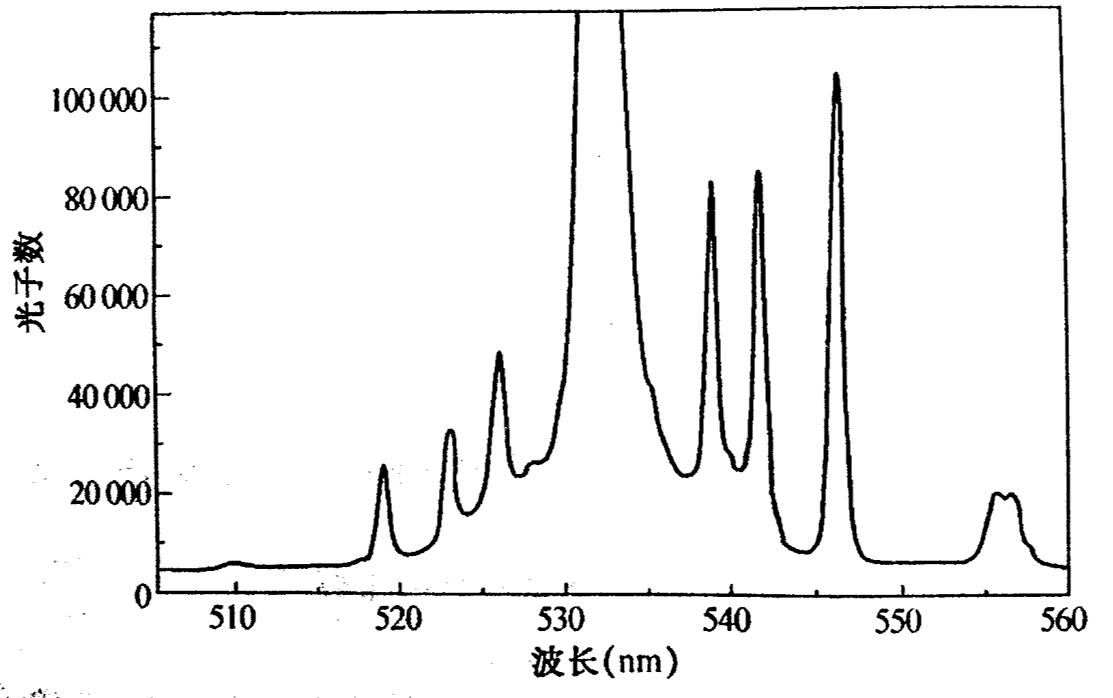
\includegraphics[width=12cm]{fig/4.png}\\
\caption{CCl$_4$分子的振动拉曼光谱}\label{fig4}
\end{figure}
\subsection{拉曼光谱的测量与分析}
拉曼光谱的测量有三种几何组态,即:直角散射、前向散射和背向散射。直角散射适用于透明晶体、透明材料的测量,前向散射用于测量研究小波矢下的声子色散关系,背向散射则适合于不透明材料的测量研究。拉曼光谱的测量如图(\ref{fig4})所示,显示了拉曼散射强度和波长(频率)之间的依赖关系,该谱的测量主要针对三个参量进行的:一是拉曼频移(化学工作者称拉曼位移),也即拉曼峰所对应的频率,通过它的测量可以研究材料的激发状况;二是线宽,即拉曼峰强度一半处的峰的全宽度,它可以给出材料的激发寿命;第三是散射强度,即拉曼峰的最大值处所对应的散射强度。频移、线宽和散射强度随参量例如温度、压力和浓度等的变化,能给出有意义的信息。
\subsection{拉曼光谱的应用}
拉曼光谱可在广泛的研究领域得到应用。比如
\begin{enumerate}
\item 相变研究:拉曼散射可以对软模、有序一无序相变、无公度相变、磁相变、液晶相变和生物相变进行研究。
\item 固体元激发研究:对极化声子、等离子体、磁振子、朗道能级分立等进行研究。
\item 体材料声子特性研究:对氧化物材料、半导体材料、髙温超导材料、高分子材料、纳米材料、矿物材料和非晶材料等拉曼谱特性进行研究。例如高温超导材料的超导相具有不同于半导体相的特征拉曼谱。
\item 表面和界面研究:表面增强拉曼散射研究吸附原子分子的物理化学特性:周期、准周期、应变层超晶格的声子特性研究、介电膜。铁电膜、光电膜、有机膜、高分子膜、生物膜等薄膜研究。
\item 微区拉曼研究:对矿物包裹体、宇宙尘、污染尘等微小样品的微区拉曼分析。
\item 生物、生化、医学等方面的研究:如蛋白质、细胞膜、DNA、线粒体电荷转移等研究,牙齿脊椎成分检测分析等。
\end{enumerate}
其他方面如:工业上煤的质量鉴定,水泥中各相成分的诊断,以及运用遥控拉曼技术对星际间氛围组成的探测,大气中水分的研究等。
\subsection{拉曼光谱的实验技术}
由于拉曼散射光强小于人射光强的10$^{-6}$倍,且比高量子效率、高电流增益的光电倍增管(PMT)的热噪声还低,故实验技术和装置都是围绕如何实现尽量增强拉曼(信号)光,抑制杂散光及将湮没于背景噪声中的信号提出设计的。为此实验采用高强度,高单色性,高方向性的激光光源,散射光收集能力强的外光路系统,利用脉冲高度甄别和数字计数技术的光子计数器。因为它输出的是脉冲信号,因而不必A/D转换,可直接送到计算机处理。图(\ref{fig5})为激光拉曼光谱仪的结构方框图。
\begin{figure}[!h]
\centering
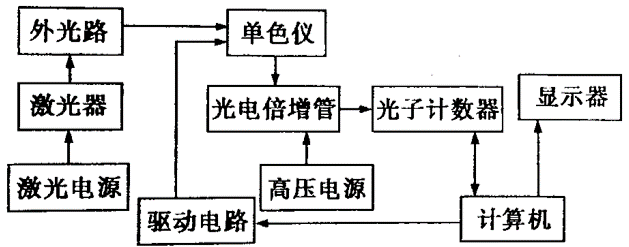
\includegraphics[width=10cm]{fig/5.png}\\
\caption{激光拉曼谱仪的结构框图}\label{fig5}
\end{figure}

\section{实验内容}
\begin{enumerate}
\item 掌握仪器的原理和技术,调节仪器至最佳状态。
\item 记录CCl$_4$分子拉曼光谱,分析辨认各谱线所对应的简正振动类型,计算分子的振动频率,计算各谱线相对于激发线的波数差。
\end{enumerate}

\section{实验数据}
\subsection{拉曼光谱图}
实验测得的拉曼光谱如图(\ref{RamanSpecFig}):
\begin{figure}[!h]
\centering
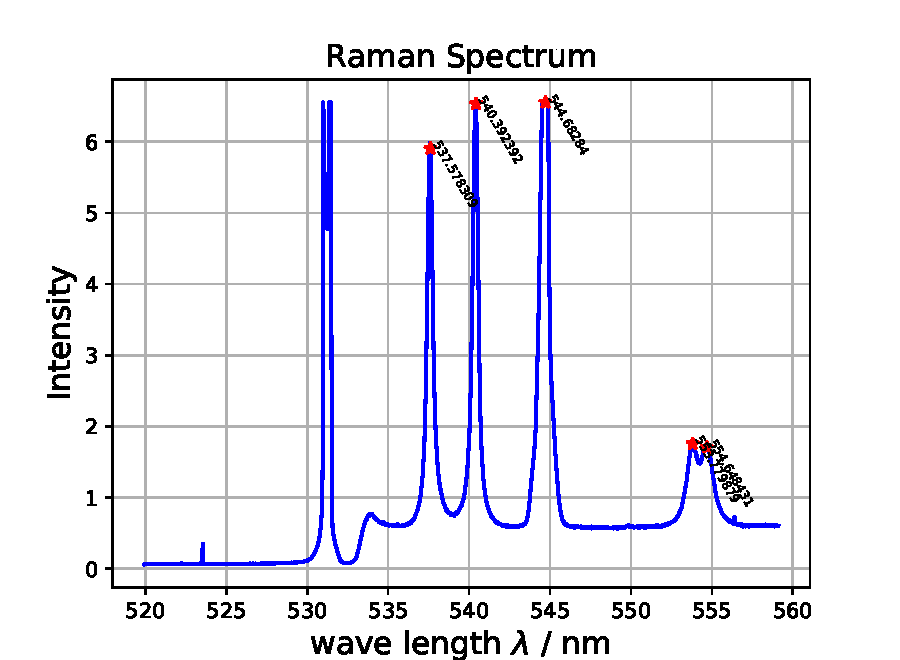
\includegraphics[width=16cm]{fig/RamanSpec.pdf}\\
\caption{$\text{CCl}_4$分子的振动拉曼光谱}\label{RamanSpecFig}
\end{figure}
\subsection{拉曼峰的数据}
从图中可观察到除了主峰外,还有四个峰,根据前文所述,可判断:\\
第三峰波长为544.68nm,是$\nu_1$\\
第二峰波长为540.39nm,是$\nu_4$\\
第一峰波长为537.58nm,是$\nu_2$\\
第四峰波长分别为553.78nm和554.65nm,是$\nu_3$。

由于我们选取的积分时间过长(约30秒),使得第二峰和第三峰的强度均达到仪器记录的最大值,无法合理地测量线宽。
\subsection{波数差}
各谱线相对于激发线(531.25nm)的波数差如下:\\
激发线波数:$k_0 = \cfrac{2\pi}{\lambda_0} \approx 11827172.34 \text{m}^{-1}$\\
第一峰波数差:$\Delta k_1 = \cfrac{2\pi}{\lambda_1} - k_0 \approx -139264.85 \text{m}^{-1}$\\
第二峰波数差:$\Delta k_2 = \cfrac{2\pi}{\lambda_2} - k_0 \approx -200041.37 \text{m}^{-1}$\\
第三峰波数差:$\Delta k_3 = \cfrac{2\pi}{\lambda_3} - k_0 \approx -291618.79 \text{m}^{-1}$\\
第四峰波数差:$\Delta k_4 = \cfrac{2\pi}{\lambda_4} - k_0 \approx -490082.39 \text{m}^{-1}$\\
注:第四峰的波数差采用了第四峰的两个小峰的平均值。

\section{实验讨论}
\iffalse
\subsection{积分时间}
实验中积分时间越长,记录的光子数越多,不同峰直接按的强度差异越明显。但是,如果积分时间过长,会导致计数仪器饱和,使得记录的光子数值一样。我们采用了30秒的积分时间,就出现了这样的问题,导致我们无法测量拉曼峰的线宽。因此,取一个合理的积分时间非常重要。
\subsection{样品气泡}
在滴加CCl$_4$样品时,我们发现极易产生气泡,必须加入略微过量的样品再推入盖玻片才能消除。同时,由于CCl$_4$挥发性很强,实验过程中可能产生气泡,若不影响测量,可以不用重新添加样品。
\fi

\section{思考题}
\subsection{为什么随着温度的升高,反斯托克斯线的强度会增大?}
\subsection{拉曼效应和荧光效应有哪些异同?}
\subsection{如何判断激光束照射CCl$_4$样品处于最佳位置?}
\subsection{为什么气体拉曼图上可以看到转动能级造成的拉曼谱线,而液体的拉曼图上一般看不到?}

\nocite{jiaocai}
\bibliography{ref}
\end{document}